\documentclass[12pt]{article}
\usepackage{color}
\usepackage{graphicx}
\usepackage{booktabs}
\usepackage{amsmath}
\usepackage[utf8]{inputenc}
%\usepackage[german]{babel}
\usepackage{multirow}
\usepackage{siunitx}
\usepackage{pbox}
%\usepackage{tabularx}
\usepackage{multirow}
\usepackage{float}
\usepackage{amssymb,amsmath}
\makeatletter
\def\maketag@@@#1{\hbox{\m@th\normalfont\normalsize#1}}
\makeatother
\setlength{\parindent}{0pt}

%\addtolength{\textwidth}{1in}
%\addtolength{\textheight}{1in}
%\addtolength{\evensidemargin}{0.5in}
%\addtolength{\oddsidemargin}{-0.5in}
%\addtolength{\topmargin}{-0.6in}
%\addtolength{\bottommargin}{0.4in}


\usepackage[top = 2.50cm, bottom = 2.50cm, left = 2.75cm, right = 2.50cm]{geometry}

\renewcommand{\floatpagefraction}{1.0}


\begin{document}
\title{PHY118/119 \\ {\bf Übungsstunde 2, Newton'sche Mechanik}}
\author{Assistent: Simon Flury \\E-mail: simon.flury@uzh.ch\\\\ }
\maketitle

\section{Wichtig!!!}
Dieses Dokument ist kein offizielles Dokument, es ist weder von Prof.Kilminster noch vom Hauptassistenten abgesegnet, somit kann sich nicht darauf bezogen werden und es wird auch keine Haftung für Fehler übernommen. Es dient einzig und allein als Lernunterstützung von mir an euch und bezieht sich ausschliesslich auf meine Übungsstunde.
\section{Newton'sche Gesetze}
Diese Woche geht es um die Einführung in die Newton'sche Mechanik, die sogenannte Kräftelehre, basierend auf den Newton'schen Axiomen.\\
\\Die Kraft ist eine vektorielle Grösse welche die Einheit Joule $J = \dfrac{kgm}{s^2}$ trägt, sie ist das Produkt aus Masse und Beschleunigung $\vec{F} = m \cdot \vec{a}$.\\
\\Die drei Newton'schen Axiomen:

\begin{itemize}
1NA (Trägheitsgesetz): Ein Körper verharrt im Zustand der Ruhe $v=0$ oder der gleichförmigen geradlinigen Translation $v=const$, sofern er nicht durch einwirkende Kräfte zur Änderung seines Zustands gezwungen wird.
\end{itemize}

\begin{itemize}
2.NA: Die Änderung der Bewegung ist der Einwirkenden Kraft proportional und geschieht in Kraftrichtung $\vec{F} = m\vec{a} = \dfrac{d}{dt} \vec{p} = \dfrac{d}{dt} m\vec{v} = m \vec{a}$
\end{itemize}
\begin{itemize}
3.NA: actio = reactio $\rightarrow$ $\vec{F}_{A\rightarrow B} = -\vec{F}_{B\rightarrow A}$
\end{itemize}

Das 2.NA sagt somit aus, das die Kraft gleich der zeitlichen Änderung des Impulses ist und somit eine Änderung der Bewegung, sprich der Geschwindigkeit darstellt (muss nicht im Betrag sein, kann auch nur eine Änderung der Bewegungsrichtung sein). Der Impuls $\vec{p} = m\vec{v}$ ist eine fundamentale Grösse in der Physik und in jedem System erhalten. Aus dem 3.NA folgt das Kräfte nur paarweise auftreten könne, somit existiert zu jeder Kraft eine Gegenkraft mit gleichem Betrag aber umgekehreten Vorzeichen.\\
\\ Es gilt das Prinzip der Superposition, dies bedeutet wirken auf einen Punkt mehrer Kräfte so addieren sich diese vektoriell zu einer resultierenden Gesamtkraft:
\begin{equation}
\vec{F}_1 + \vec{F}_2 +...+ \vec{F}_n = \sum_{i=1}^n \vec{F}_i = \vec{F}_{res}
\end{equation}
Ist das System statisch, also bewegt sich der Körper nicht, so gilt $\vec{F}_{res} = 0 $, ist das System dynamisch, also bewegt sich der Körper so gilt $\vec{F}_{res} \ne 0$, dementsprechend wirkt eine resultierende Beschleunigung und der Körper erhält somit eine Geschwindigkeit in eine Richtung. Bei den Betrachtungen die wir momentan tätigen, greiffen die Kräfte immer im Schwerpunkt des Körpers an, ist dies nicht der Fall führt dies zu einem sogenannten Drehmoment (kommt später in der Vorlesung noch).
\\
\\
Bewegt sich ein Körper auf einer Kreisbahn erfährt er zwei Beschleunigungen, eine tangentiale $a_{\varphi}$ und eine zum Zentrum gerichtete, die sogenannte Zentripetalbeschleunigung $a_r = \dfrac{v^2}{R}$
\begin{figure}[H]
  \centering{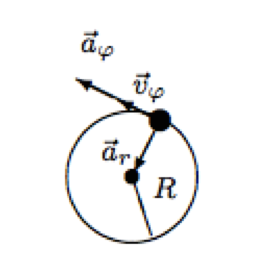
\includegraphics[width=0.4\textwidth]{Kreisbahn.png}}
  \caption{Beschleunigungen auf Kreisbahn}
  \label{fig:1teil}
\end{figure} 
Merkt euch, da eine Beschleunigung auf eine Masse wirkt, wirkt eine Kraft, die sogennate Zentripetalkraft $F_r = m \cdot a_r$. Um dies noch anders schreiben zu können führen wir die Winkelgeschwindigkeit ein:
\begin{itemize}
$\dot{\varphi} = \omega$ ist die Winkelgeschwindigkeit 
\end{itemize}
\begin{itemize}
$\ddot{\varphi} = \dfrac{d\omega}{dt} = \beta$ ist die Winkelbeschleunigung
\end{itemize}
diese grössen beschreiben die zeitliche Änderung eines Winkels, also welche Winkeldifferenz wird in einem gewissen Zeitintervall überstrichen.
Mit diesen neuen Grössen kann man schreiben:
\begin{equation}
a_r = \dfrac{v^2}{R} = \omega^2R
\end{equation}
\begin{equation}
a_{\phi} = R\dfrac{d^2\varphi}{dt^2} = R\beta
\end{equation}
Bitte seit euch bewusst, dass diese beiden Beschleunigungen senkrecht aufeinander stehen! (ist dies nicht klar fragt mich bitte in der Übungsstunde).\\
\\
Die Zentrifugalkraft ist vom Betrag her gleich der Zentripetalkraft, einfach vom Zentrum nach aussen gerichtet, also mit umgekehrten Vorzeichen. Diese Kraft ist jedoch nur ein kinematisches Produkt, eine Scheinkraft. Dies bedeutet, dass sie vom Bezugssystem abhängt indem man sich befindet, bei einer Kreisbewegung befinden wir uns in einem beschleunigten Bezugssystem. Geht man über in ein Inertialsystem verschwinden die Scheinkräfte. (Ich weiss nicht ob diese Begriffe in der Vorlesung eingeführt wurden, fals nicht kann ich sie euch in der Stunde kurz erklären, oder ihr könnt diesen Beitrag getrost ignorieren ;) )

\section{Wahrscheinlichkeitsverteilungen}
In der Vorlesung habt ihr zwei Arten von Wahrscheinlichkeitsverteilungen kennen gelernt, die Binimonalverteilung und die Gaussverteilung (Normalverteilung)\\
\\Binominalverteilung: Gibt Wahrscheinlichkeit für k-mal ein positives Ergebnis aus n Versuchen. Das bedeutet, der Ausgang jedes einzelnen Versuchs ist entweder positiv oder negativ.
\begin{equation}
P(k|p,n) = \binom{n} {k} p^k(1-p)^{n-k}
\end{equation}
wobei $p$ die Wahrscheinlichkeit für ein positives Ereignis angibt, $k$ die Anzahl positiver Ereignisse, $n$ Anzahl Versuche. Somit besteht diese Gleichung aus dem Binominalkoeffizienten $\binom{n} {k} = \dfrac{n!}{k!(n-k)!}$, der Wahrscheinlichkeit für k mal ein positives Ereignis $p^k$,  multupliziert mit $n-k$ mal der Wahrscheinlichkeit für ein negatives Ereignis $(1-p)^{n-k}$.
\\
\\ Beispiel: Ihr Werft 20mal eine Münze und wollt wissen wie gross die Wahrscheinlichkeit ist 5mal Kopf zu erhalten.\\
Nun ist $n=20$, $k=5$ und $p=1/2$
\begin{equation}
P(5|1/2,20) = \binom{20} {5} 1/2^5(1-1/2)^{20-5} \approx 0.015 = 1.5\%
\end{equation}
\\
\\
Gaussverteilung: Gibt Wahrscheinlichkeit für einen bestimmtes Ereignis x, in einen Zufallsexperiment an.
\begin{equation}
p(x|\mu,\sigma) = \dfrac{1}{\sqrt{2\pi \sigma^2}} \cdot exp\left(-\dfrac{(x-\mu)^2}{2\sigma^2} \right)
\end{equation}
dabei steht $\mu$ für den Mittelwert und $\sigma$ für die Standardabweichung. (Erinnert euch an Aufgabe 5 aus Serie 2, dort war der Mittelwert $\mu = 110km/h$ und die Standardabweichung $\sigma = 10km/h$

\begin{figure}[H]
  \centering{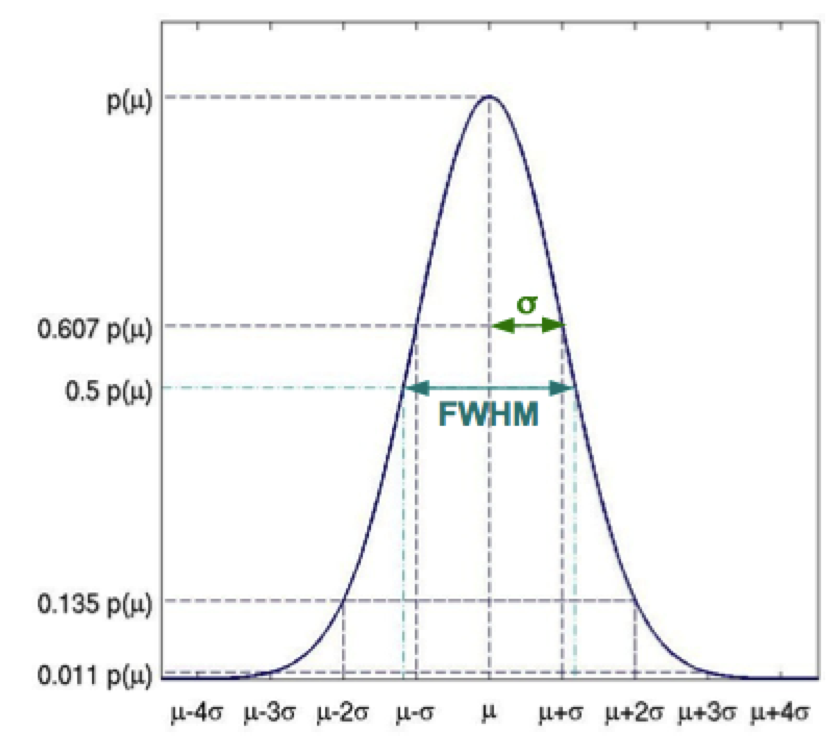
\includegraphics[width=0.7\textwidth]{Gauss.png}}
  \caption{Gaussverteilung, FWHM bedeutet Full Width at Half Maximum (Breite der Verteilung auf halber Höhe.)}
  \label{fig:1teil}
\end{figure} 

 Wie ihr seht ist diese Funktion ein wenig kompliziert, was ihr euch jedoch einfach merken könnt sind die jeweiligen Wahrscheinlichkeiten für $\pm \sigma$ sowie die Tatsache das die Funktion symmetrisch um den Mittelwert ist.
\begin{itemize}
$P(|x-\mu| \le 1\sigma) = 68.27\%$
\end{itemize}
\begin{itemize}
$P(|x-\mu| \le 2\sigma) = 95.45\%$
\end{itemize}
\begin{itemize}
$P(|x-\mu| \le 3\sigma) = 99.73\%$
\end{itemize}
  \label{fig:1teil}
\end{figure} 

\end{document}
